\begin{graphicspathcontext}{{./chapters/hmas/imgs/},{./chapters/hmas/imgs/auto/},\old}

\begin{frame}{Holon Concept}
	\begin{columns}
		\begin{column}{.5\linewidth}
			\begin{definitionblock}{Holon \cite{koestler67}}
				A \Emph{holon} is an entity that is simultaneously:
				\begin{description}
				\item[A whole] it has its own identity, autonomy and behaviour (seen from the outside as a single agent)
				\item[A part] it is a member of a larger holon (seen from the outside as a component of a system)
				\end{description}
			\end{definitionblock}
			\vspace{.25cm}
			\begin{block}{Dual nature}
				From the \emph{outside}: an \Emph{agent} \\
				From the \emph{inside}: a \Emph{multi-agent system}
			\end{block}
		\end{column}
		\begin{column}{.5\linewidth}
			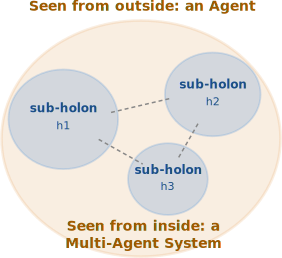
\includegraphics{hmas_holon_dual_nature}
		\end{column}
	\end{columns}
\end{frame}

\sidecite{koestler67}
\begin{frame}{Properties of a Holon}
	\begin{block}{Four fundamental properties}
		\begin{description}
		\item[Self-similarity] A holon is structurally similar to its sub-holons; the same organisational patterns repeat at every level
		\item[Autonomy] Each holon can operate independently; it has its own goals, resources, and decision-making processes
		\item[Cooperativity] A holon cooperates with other holons at the same level and contributes to the goals of its super-holon
		\item[Recursiveness] The composition relationship applies recursively: a sub-holon may itself contain holons
		\end{description}
	\end{block}
	\vspace{.25cm}
	\begin{exampleblock}{Analogy}
		A \emph{cell} is a self-contained living entity \emph{and} a part of a tissue, which is a part of an organ, which is part of an organism
	\end{exampleblock}
\end{frame}

\begin{frame}{What is a Holarchy?}
	\begin{columns}
	\begin{column}{.6\linewidth}
		\begin{definitionblock}{Holarchy \cite{koestler67}}
			A \Emph{holarchy} is the hierarchical structure formed by the \Emph{part-of} relationships between holons
		\end{definitionblock}
		\vspace{.25cm}
		\begin{block}{Properties of a holarchy}
			\begin{description}
			\item[No absolute bottom] a leaf can always be decomposed further
			\item[No absolute top] any super-holon may itself be a part of another
			\item[Level of observation] determines what appears as atomic
			\item[Emergent properties] arise from the interactions within a holon
			\end{description}
		\end{block}
	\end{column}
	\begin{column}{.4\linewidth}
		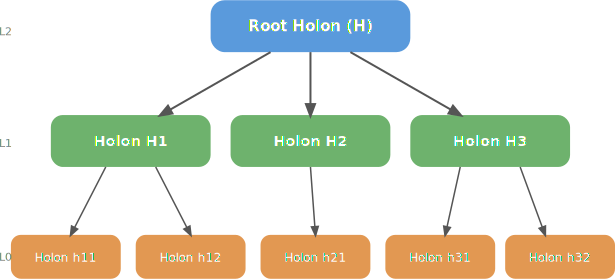
\includegraphics{hmas_holarchy}
	\end{column}
	\end{columns}
\end{frame}

\figureslide{{Holarchy:} an example}{holonic-organizational-decomposition}

\begin{frame}{Holarchy vs.\ Classical Hierarchy}
	\begin{stabularx}{X|X|X}
	\tabularhead{Aspect}{Classical Hierarchy}{Holarchy} \\
	Nature of nodes & Passive components & Autonomous agents \\
	\hline
	Direction & Top-down control & Both directions   \\
	\hline
	Boundaries & Fixed, absolute & Relative to level \\
	\hline
	Composition & Static & Dynamic           \\
	\hline
	Emergence & Not modelled & First-class concept \\
	\hline
	Granularity & Fixed decomposition & Level of observation \\
	\end{stabularx}
\end{frame}

\end{graphicspathcontext}

\endinput

